% ---------------------------- Preamble starts here ----------------------------

\documentclass[aspectratio=169]{beamer} %Remove [aspectratio=169] to get non-wide 4:3 slide aspect ratio

% --- Set beamer theme
\usetheme{Metropolis}
\setbeamertemplate{footline}{}				% Remove automatic footer
\setbeamertemplate{navigation symbols}{}	% Comment this line to display navigation symbols

% Load i2i symbol
\addtobeamertemplate{frametitle}{}{%
\begin{textblock*}{\linewidth}(0cm,7.4cm) % Replace with (0cm, 8cm) if using non-wide slide aspect
	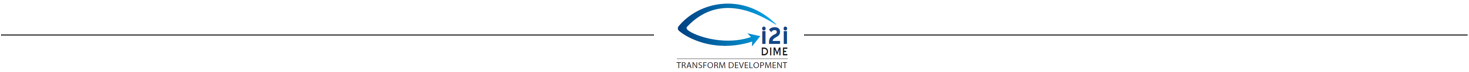
\includegraphics[width=\linewidth]{../../Common-Resources/img/Footer.png}
\end{textblock*}}

% --- Load packages
\usepackage{textpos}		% To align objects correctly
\usepackage{multicol}		% To right in multiple columns
\usepackage{color}			% To color text

% --- Add your information here
\title{An intro to Git and GitHub - Observer Role}
\author{DIME Analytics}
\institute{DIME - The World Bank}
\date{\today}

\newcommand{\trainingURL}[1]{{\color{blue}\url{#1}}}

\newcommand{\traininerUsername}{kbjarkefur}
\newcommand{\repoName}{\traininerUsername/country-facts}
\newcommand{\trainingRepoURL}[1]{\trainingURL{github.com/\repoName #1}}
\newcommand{\trainerEmail}{\trainingURL{kbjarkefur@worldbank.org} }

% ---------------------------- Preamble ends here ----------------------------

\begin{document}

\begin{frame}

\includegraphics[width=\textwidth]{../../Common-Resources/img/Header.png}
\vspace{-0.2cm}
\titlepage 	 % Opening slide, prints inform
\end{frame}

\begin{frame}
\frametitle{Before the session starts:}
	\begin{enumerate}
		\item Do you have a GitHub.com account? If not, got to \trainingURL{https://github.com/join} and sign up
		\item Open \trainingRepoURL{} in a browser
	\end{enumerate}
\end{frame}

\begin{frame}

\includegraphics[width=\textwidth]{../../Common-Resources/img/Header.png}
\vspace{-0.2cm}
\titlepage 	 % Opening slide, prints inform
\end{frame}

\begin{frame}
	\frametitle{Three common GitHub roles}
	
	\small The objective of this training is to make you able to take the role of an \textbf{Observer}. See DIME Analytics GitHub Roles for full details (link in end of presentation).
	
	

\begin{columns}[T] 
	\column{.33\textwidth} % Left column and width
	\Large \center{\textbf{Observer}}
	\begin{itemize}
		\small \item Browse code in GitHub
		\small \item Provide feedback through GitHub
		\small \item \textbf{Who?} Typically a PI that does not code
	\end{itemize}
	
	\column{.33\textwidth} % Middel column and width
	\Large \center{\textbf{Contributor}}
	\begin{itemize}
		\small \item Contribute to code in GitHub
		\small \item Understand and follow instructions from a Repo Maintainer
		\small \item \textbf{Who?} Typically an RA, or a PI that codes
	\end{itemize}
	
	\column{.33\textwidth} % Right column and width
	\Large \center{\textbf{Repo Maintainer}}
	\begin{itemize}
		\small \item Make sure that best practices and standards are followed in the repository
		\small \item Guide new contributors
		\small \item \textbf{Who?} Typically the most senior RA. Takes too much time for a PI.
	\end{itemize}
	
\end{columns}
	




\end{frame}

\begin{frame}
\frametitle{What is Git used for?}

	\begin{columns}[c] 
		
		\column{.60\textwidth} % Left column and width
		\begin{itemize}
			\item Git solves the \textit{Final.doc} problem
			\item <2->Common solution to the \textit{Final.doc} problem. Name all your docs like \textit{YYMMDD\_docname\_INITIALS.doc}
			\item <3->Git tracks \textit{YYMMDD} and \textit{INITIALS} for all edits  without the user having to remember it
			\item <4->That's far from everything, Git also solves:
			\begin{itemize}
				\item <4->Conflicting copy problem (DropBox etc.)
				\item <4->I can't re-produce my Baseline report problem
				\item <4->Who wrote this code 4 years ago and why?
				\item <4->And much much more...
			\end{itemize} 
		\end{itemize}	
		
		\column{.40\textwidth} % Right column and width
		\begin{figure}
			\centering
			
\includegraphics[width=1\linewidth]{../../Common-Resources/img/finaldoc_cartoon}
			\label{fig:finaldoccartoon}
		\end{figure}
		
	\end{columns}
\end{frame}

\section{Git vs. GitHub vs. GitHub Desktop}

\begin{frame}
	\frametitle{What is Git, GitHub and GitHub Desktop?}
	\begin{figure}
		\centering
		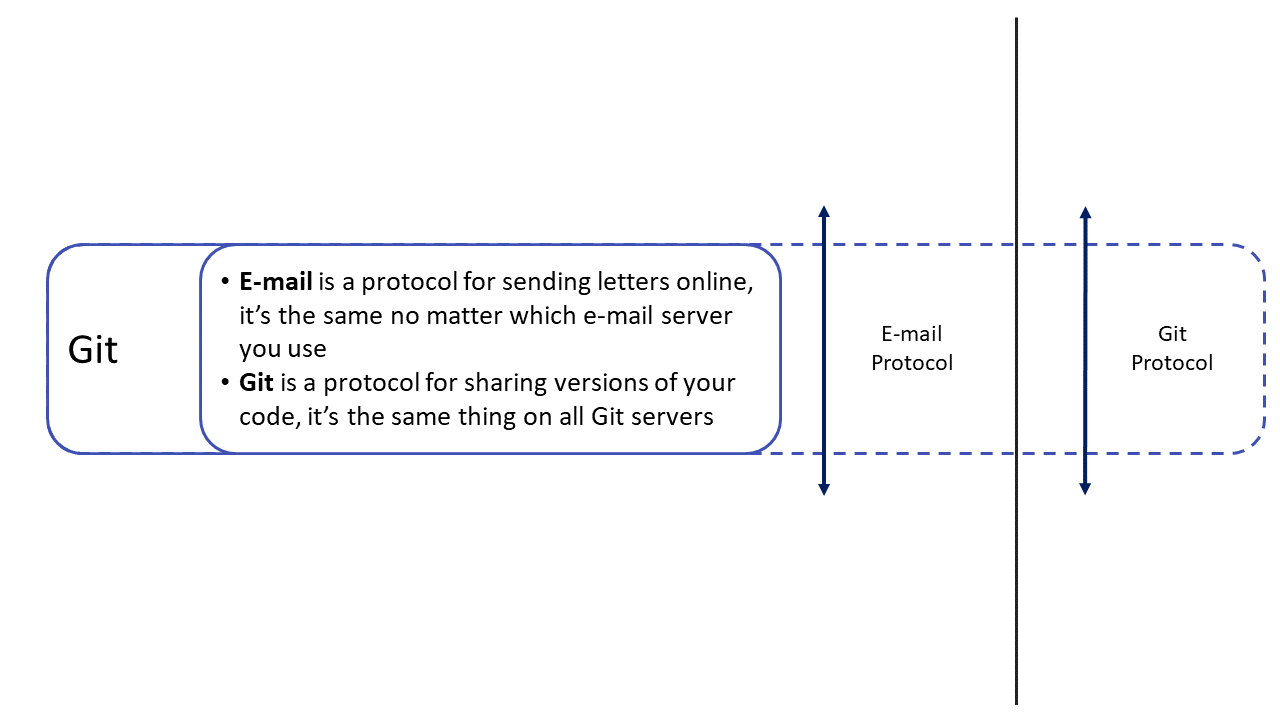
\includegraphics[width=0.7\linewidth]{../../Common-Resources/img/git_github_gitclient_git}
		\label{fig:gitgithubgitclient_git}
	\end{figure}
\end{frame}

\begin{frame}
	\frametitle{What is Git, GitHub and GitHub Desktop?}
	\begin{figure}
		\centering
		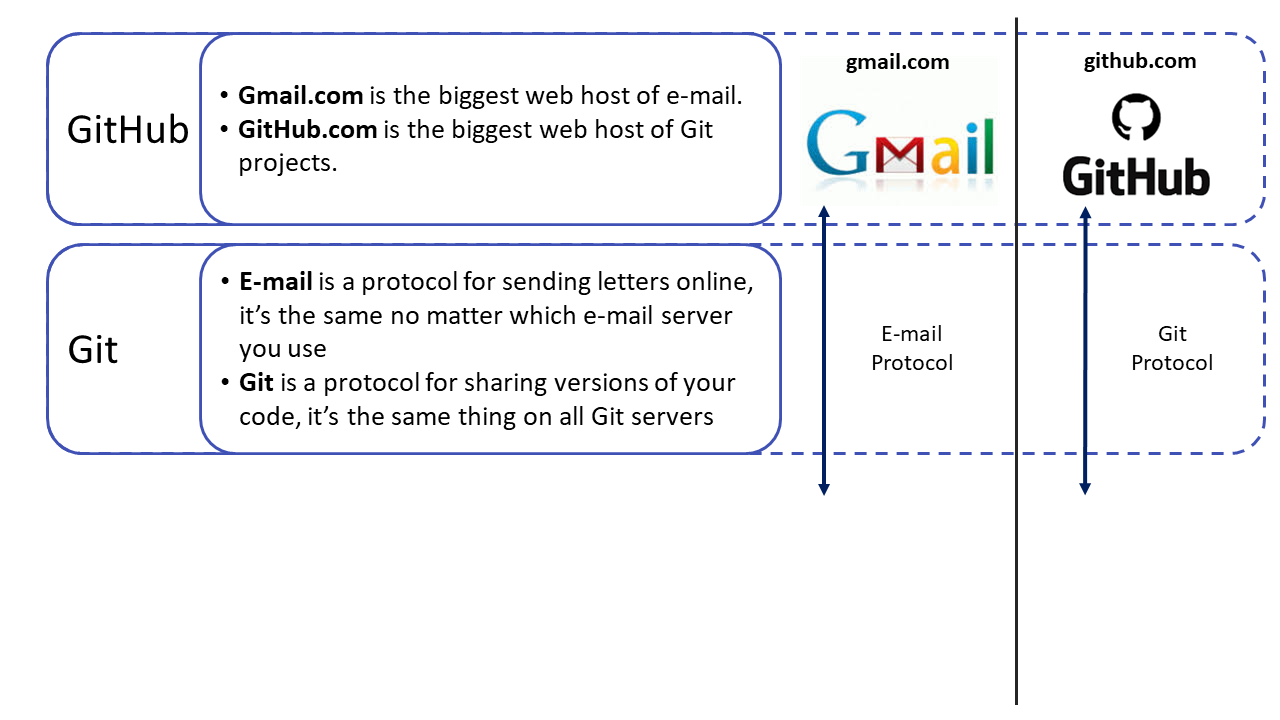
\includegraphics[width=0.7\linewidth]{../../Common-Resources/img/git_github_gitclient_github}
		\label{fig:gitgithubgitclient_github}
	\end{figure}
\end{frame}

\begin{frame}
	\frametitle{What is Git, GitHub and GitHub Desktop?}
	\begin{figure}
		\centering
		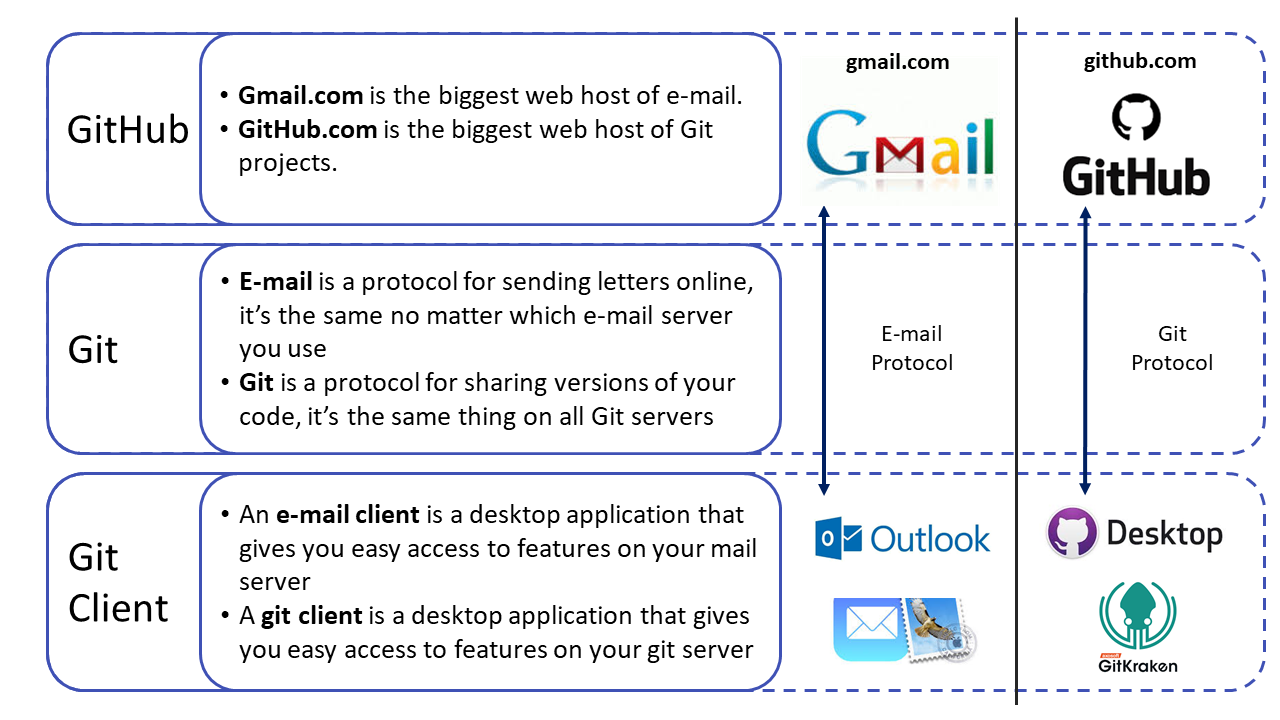
\includegraphics[width=0.7\linewidth]{../../Common-Resources/img/git_github_gitclient_gitclient}
		\label{fig:gitgithubgitclient_gitclient}
	\end{figure}
\end{frame}




\section{Exploring a Repository}

\begin{frame}
	\frametitle{Today's objective - 7 min}
	
	\begin{columns}[c] 
		
		\column{.15\textwidth} % Left column and width
		
		\column{.70\textwidth} % Left column and width
		
		\Large{What we will cover today:}
		
		\vspace{.5cm}
		
		\begin{itemize}
			\large{\item Browse code on GitHub}
			\begin{itemize}
				\normalsize{\item \textbf{Commits} - very briefly}
				\normalsize{\item \textbf{Branches} - very briefly}			
			\end{itemize}
			\large{\item Provide feedback through GitHub}
			\begin{itemize}
				\normalsize{\item \textbf{Issues}}		
			\end{itemize}		
			\large{\item Discuss some basic GitHub best practices}
		\end{itemize}
		
		\column{.15\textwidth} % Left column and width
		
	\end{columns}
\end{frame}

\begin{frame}
	\frametitle{How to browse GitHub.com}
	
	Your project folder is called a \textbf{repository} in Git. We will call the page you land on when you enter \trainingRepoURL{} the \textbf{main page}.
	
	\vspace{.5cm}
	
	\begin{columns}[T] 
		
		\column{.50\textwidth} % Left column and width
		GitHub.com -$>$ Repo
		\begin{enumerate}
			\item From anywhere on \trainingURL{github.com} click the \textit{octocat} icon in the top left corner.
			\item In the menu to your left you see the repositories you are invited to
			\item Click any repo to get to the main page of that repo.
		\end{enumerate}
		
		\column{.50\textwidth} % Left column and width
		Repo -$>$ Main page
		\begin{enumerate}
			\item Click the repo name in \trainingURL{\repoName} at the top of any page within the repo
			\item Click the tab that says \textbf{Code} below the repo name at any page in your repo
		\end{enumerate}
		
	\end{columns}
\end{frame}


\begin{frame}
	\frametitle{Country Facts!}
	
	\begin{columns}[c] 
		
		\column{.10\textwidth} % Left column and width
		
		\column{.80\textwidth} % Left column and width
		\textbf{No focus on code today!}
		
		\vspace{.25cm}
		
		Code tends to distract people if, for example, they see a command they do not understand. Instead we will work on a \textit{Country Fact Sheet} in a file called \textit{countries.do}. 
		
		\vspace{.25cm}
		
		It is a .do file, so the content will behave just as code, but there is no code in it.

		\vspace{.25cm}

		We will look at some examples that uses actual code once we are familiar with the features we will cover today. 
		
		\column{.10\textwidth} % Left column and width
		
	\end{columns}
	
	\vspace{.55cm}
	\trainingRepoURL{/blob/master/facts/countries.do}
		
	
\end{frame}

\begin{frame}
	\frametitle{In-depth}

	\begin{columns}[c] 
	
	\column{.10\textwidth} % Left column and width
	
	\column{.70\textwidth} % Left column and width
	
		You are not expected to get a full understanding of \textbf{Commits} and \textbf{Branches} and how they are used today, that is what the \textit{Contributor training} is for. 
		
		\vspace{.5cm}
		
		But after I have briefly covered these two topics and also introduced \textbf{Issues}, we will look at an example that will give you the intuition for what \textbf{Commits} and \textbf{Branches} are.
		
	\column{.15\textwidth} % Left column and width

	\end{columns}		
		
\end{frame}


\section{Commits}

\begin{frame}
	\frametitle{What is a commit? - 12 min}

	\begin{columns}[c] 
	
		\column{.45\textwidth}
		\textbf{In DropBox}, each saved version of a file is saved to the version history. Are all these versions meaningful differences? 
		
		\vspace{.35cm}
		
		\textbf{In GitHub}, commits are used to indicate what is a meaningful difference. 
		
		\vspace{.35cm}
		
		One meaningful difference can be large or small, can be an edit to one, some or all files at the same time.
		
		\column{.55\textwidth}
		\begin{figure}
			\centering
			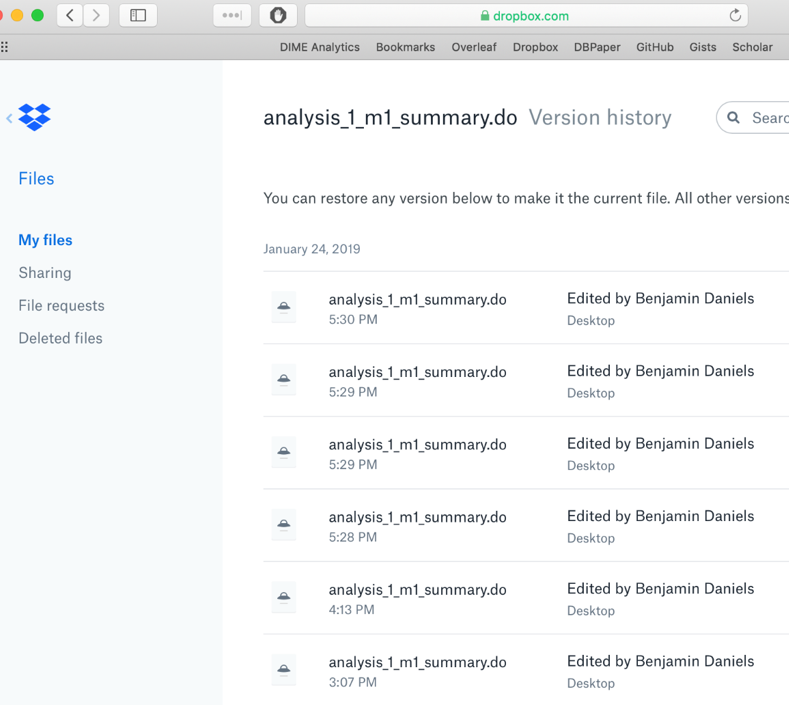
\includegraphics[width=1\linewidth]{../../Common-Resources/img/dropbox_versioncontrol}
			\label{fig:dropboxversioncontrol}
		\end{figure}
		
	\end{columns}
\end{frame}

\begin{frame}
	\frametitle{Exploring commits}

	Now when have a basic understanding of what a \textit{Commit} is, we can start exploring how the \trainingRepoURL{} repository was created.
	
	\vspace{.25cm}
	
	We will see a list of commits, that at first sight is similar to the the version history in DropBox, but \textbf{in Git the version list is more meaningful, as it is a list of only meaningful differences}.

	\vspace{.25cm}
	
	\begin{itemize}
		\item \trainingRepoURL{/commits}
	\end{itemize}	

\end{frame}

\section{Branches}

\begin{frame}
	\frametitle{Introducing branches  - 16 min}

	\begin{columns}[c] 
		
		\column{.60\textwidth}
		\textbf{Branches is the "killer feature" of Git}. This is where Git becomes really powerful as a collaboration tool and as version control.
		
		\vspace{.25cm}
	
		Branches allows you to \textbf{create a copy of the code where you can experiment}, if you like the result, \textbf{you can very easily merge your experiment with the main version of your code}.
		
		\vspace{.25cm}
		
		This non-linear version control is much more similar to how we actually work than the strictly linear version control in, for example, DropBox
		
		\column{.40\textwidth}
		\begin{figure}
			\centering
			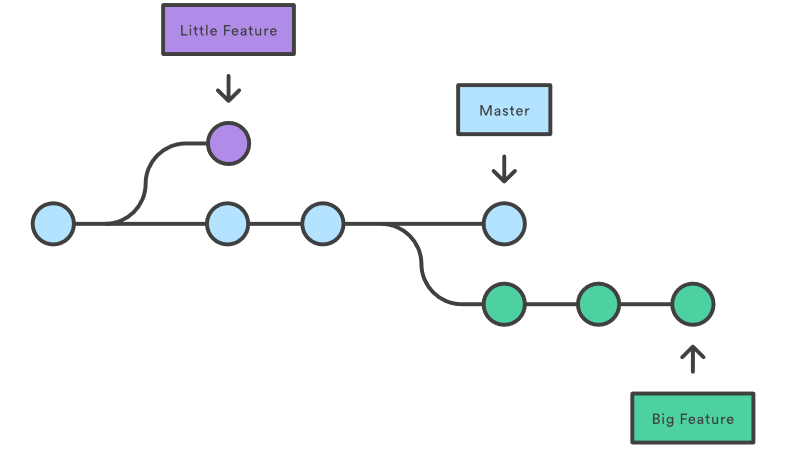
\includegraphics[width=1\linewidth]{../../Common-Resources/img/branches}
			\label{fig:branches}
		\end{figure}
		
	\end{columns}
\end{frame}

\begin{frame}
	\frametitle{Looking at branches}

	\textbf{One more way to explore the repository}
	\begin{itemize}
		\item \trainingRepoURL{/commits} $<$- Linear progression
		\item \trainingRepoURL{/network} $<$- Non-linear progression
	\end{itemize}
\end{frame}

\section{Issues}

\begin{frame}
	\frametitle{Issues are feedback - 20 min}
	
	\textbf{Issues are optional} in Git/GitHub, you do not have to use them
	
	\vspace{.20cm}
	
	\textbf{Issues} in GitHub is where you discuss \textbf{feedback}. It is like a \textbf{task management tool integrated with your code}
	
	\vspace{.20cm}
	
	\textbf{Issues and edits to the code can be linked} so that anyone with access to the repo, can \textbf{link a discussion about an edit to the code to the Commit with that edit}
	
	\vspace{.20cm}
	
	The link can also goes the other way, so \textbf{if Commits and Issues are linked}, then anyone in the future with access to the repo, can \textbf{link edits to the code in a Commit with the discussions that lead up to that edit}
	
	\vspace{.20cm}
	
	Resolved \textbf{Issues are archived and searchable on GitHub} as long as the repo exists
\end{frame}

\begin{frame}
	\frametitle{Issues are feedback}
	
	For each \textit{Issue} \textbf{a discussion thread} will be opened where anyone with access to the repo can contribute to the discussion

	\vspace{.25cm}
	
	Issues can be \textbf{assigned} to GitHub users similarly to a task management tool
	
	\vspace{.25cm}
	
	Specific \textbf{lines of code can be referenced and previewed}, so the discussion can be tied to specific lines of code, making it clear to everyone what is being discussed
	
	\vspace{.25cm}
	
	In addition to reference specific lines of code, there are tools to \textbf{label} \textit{Issues}, \textbf{cross reference} \textit{Issues}, \textbf{tag people} relevant to the discussion etc. so that collectively the \textit{Issues} becomes a the \textbf{documentation} or the meta-information on how the code for your project was developed
\end{frame}

\begin{frame}
	\frametitle{Commits - Branches - Issues}
	\center{
		\Large{An example that ties commits, branches and issues together:}
		
		\vspace{.5cm}
		\normalsize{Go to the issues tab, then click the issue with the title \textbf{Capital of India is incorrect}. 
			
		Or type this URL in your browser: \trainingRepoURL{/issues/1}}
	}
	\vspace{1cm}
	
\end{frame}

\section{Practice issues}

\begin{frame}
	\frametitle{How to create an issue - 27 min}
	
	Time to create issues! Go to: \trainingRepoURL{/blob/master/facts/countries.do}	
	\vspace{.5cm}

	\begin{columns}[c] 
	
		\column{.60\textwidth}	
		\begin{enumerate}
			\item Find an incorrect fact to create an issue for
			\item Click the line number of the line with the incorrect fact you want corrected
			\item Click the three-dot menu that appears
			\item Click \textit{Reference in new issue}
			\item Give the issue a title, describe what you want fixed, use the \textit{preview} as needed, and then click \textit{Submit new issue}
		\end{enumerate}	
	
		\column{.40\textwidth}
		\begin{figure}
			\centering
			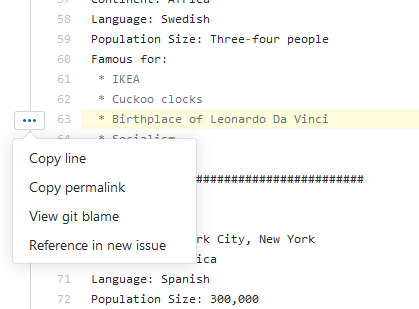
\includegraphics[width=1\linewidth]{img/reference-code-line-issue.png}
			\label{fig:branches}
		\end{figure}
	\end{columns}
\end{frame}

\begin{frame}
	\frametitle{Interact with issues}
	
	\begin{columns}[c] 
		
		\column{.15\textwidth}
		
		\column{.70\textwidth}	
		\begin{enumerate}
			\item Assign me (\textit{\traininerUsername}) or someone else to the \textit{Issue} you just created
			\item See if you find a label that fit your \textit{Issue}
			\item Write a comment on an \textit{Issue} someone else created
			\item Click the \textbf{Subscribe} button on an issue that you have not interacted with. This will give you notification on activities in this issue. 
		\end{enumerate}	
		
		\column{.15\textwidth}

	\end{columns}
\end{frame}

\begin{frame}
	\frametitle{Multi-line code reference}
	
	How to reference multiple lines of code:
	\vspace{.5cm}
	
	\begin{columns}[T] 
		
		\column{.45\textwidth}
		\textbf{Using menus:}
		\begin{enumerate}
			\item Click the line number of the first line you want to reference
			\item Before clicking the three-dot menu that appears, hold shift and click the last line you want to reference
			\item Then click the three-dot menu and click \textit{Reference in new issue}
		\end{enumerate}	
		
		\column{.55\textwidth}
		\textbf{Manually:}
		\begin{enumerate}
			\item Create a one line reference and edit the link from: {\color{blue}https://}\trainingRepoURL{/blob/random-sha/facts/countries.do\#L18}
			\item Modify the end of the URL to: {\color{blue}https://}\trainingRepoURL{/blob/random-sha/facts/countries.do\#L18-L22}
		\end{enumerate}	
	\end{columns}
\end{frame}

\begin{frame}
	\frametitle{Multiple code references}
	
	How to reference multiple lines of code: 
	\vspace{.5cm}
	
	\begin{columns}[c] 
		
		\column{.60\textwidth}	
		\textbf{No way to do this in menus}
		\begin{enumerate}
			\item When you click \textit{Reference in new issue} GitHub copies a permalink to the code line and put that in an issue
			\item In the menu in the three-dot menu you can instead click \textit{Copy permalink}. This creates the same link as when clicking \textit{Reference in new issue}. 
			\item Create an issue an copy permalinks to all code lines that you want to reference and copy them to the issue
		\end{enumerate}	
		
		\column{.40\textwidth}
		\begin{figure}
			\centering
			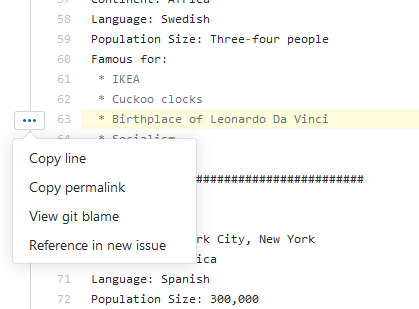
\includegraphics[width=1\linewidth]{img/reference-code-line-issue.png}
			\label{fig:branches}
		\end{figure}
	\end{columns}
\end{frame}

\section{Where are files when using Git/GitHub?}

\begin{frame}
	\frametitle{Where should I look for ...? - 40 min}
	
	\begin{columns}[c] 
	
		\column{.10\textwidth}
		
		\column{.60\textwidth}	
		\Large Your project is now using GitHub, where should I look for:
		
		\vspace{0.5cm}
		
		\begin{itemize}
			\item code?		
			\item data? 
			\item outputs?		
		\end{itemize}
		
		\column{.30\textwidth}
		
	\end{columns}	
\end{frame}

\begin{frame}
	\frametitle{Where should I look for code?}
	
	Where should I look for \textbf{code}?
	
	\begin{itemize}
		\item Code is now in Git/GitHub. 
		\begin{itemize}
			\item It is error prone to also keep it on DropBox
			\item No problem to have archived copies of code on DropBox, just don't do work on them
		\end{itemize}
		\item How to access code:
		\begin{itemize}
			\item \textbf{Browser:} Go to the URL of your repository and explore code using your browser
			\item \textbf{Download for collaboration:} Clone the repository. It is covered in the collaborator training.
		\end{itemize}		
	\end{itemize}
\end{frame}

\begin{frame}
	\frametitle{Where should I look for data?}
	
	Where should I look for \textbf{data}?
	
	\begin{itemize}
		\item Data is where it was before (ex. DropBox). 
		\begin{itemize}
			\item Github is secure, but not secure enough for project data
			\item Most data formats is not suited for GitHub and makes GitHub slow
		\end{itemize}
		\item How to access data:
		\begin{itemize}
			\item Same as before.
			\item Code reads data from DropBox, and reads code from the clone.
		\end{itemize}		
	\end{itemize}
\end{frame}

\begin{frame}
	\frametitle{Where should I look for outputs?}

	Where should I look for \textbf{outputs}?
	
	\begin{itemize}
		\item Outputs can go both on Git/GitHub and on DropBox. It is up to the project team!
		\item GitHub/Git:
		\begin{itemize}
			\item \textbf{Pro:} Tables in .txt/.tex and other raw text formats can be tracked in Git and differences between version will be displayed
			\item \textbf{Con:} Outputs are not available on DropBox without an extra step
		\end{itemize}
		\item DropBox
		\begin{itemize}
			\item \textbf{Pro:} Outputs become available immediately for everyone
			\item \textbf{Con:} If two branches creates different outputs, they will overwrite each other's output, with no documentation on which branch the output came from
		\end{itemize}		
	\end{itemize}
\end{frame}


\section{Other tools good for management}

\begin{frame}
	\frametitle{Blame  - 43 min}
	
	Have you ever looked at code you or someone in your project wrote asking yourself these questions:
	
	\begin{itemize}
		\item Who wrote this line of code?
		\item When did someone write this line of code?
		\item Why did someone write this line of code?		
	\end{itemize}	
	
	Git has a feature for this \textit{"tactfully"} called \textbf{Blame}.
	
	\begin{itemize}
		\item \trainingRepoURL{/blame/master/facts/countries.do}
	\end{itemize}
\end{frame}

\begin{frame}{Useful links}
	\begin{itemize}
	  \item All DIME Analytics GitHub resources: \trainingURL{https://github.com/worldbank/dime-github-trainings}. For example:
		\begin{itemize}
			\item DIME Analytics GitHub Templates (for example .gitignore): \trainingURL{https://github.com/worldbank/dime-github-trainings/tree/master/GitHub-resources/DIME-GitHub-Templates}
			\item DIME Analytics GitHub Roles: \trainingURL{https://github.com/worldbank/dime-github-trainings/blob/master/GitHub-resources/DIME-GitHub-Roles/DIME-GitHub-roles.md}
		\end{itemize}
		\item Markdown cheat sheet (how to format text on GitHub.com):  \trainingURL{https://www.markdownguide.org/cheat-sheet/}
		\item DIME GitHub Account admin info and instructions: \trainingURL{https://github.com/dime-worldbank/dime-account-admin}
	\end{itemize}
\end{frame}


\end{document}
